% Options for packages loaded elsewhere
\PassOptionsToPackage{unicode}{hyperref}
\PassOptionsToPackage{hyphens}{url}
%
\documentclass[
]{article}
\usepackage{amsmath,amssymb}
\usepackage{lmodern}
\usepackage{iftex}
\ifPDFTeX
  \usepackage[T1]{fontenc}
  \usepackage[utf8]{inputenc}
  \usepackage{textcomp} % provide euro and other symbols
\else % if luatex or xetex
  \usepackage{unicode-math}
  \defaultfontfeatures{Scale=MatchLowercase}
  \defaultfontfeatures[\rmfamily]{Ligatures=TeX,Scale=1}
\fi
% Use upquote if available, for straight quotes in verbatim environments
\IfFileExists{upquote.sty}{\usepackage{upquote}}{}
\IfFileExists{microtype.sty}{% use microtype if available
  \usepackage[]{microtype}
  \UseMicrotypeSet[protrusion]{basicmath} % disable protrusion for tt fonts
}{}
\makeatletter
\@ifundefined{KOMAClassName}{% if non-KOMA class
  \IfFileExists{parskip.sty}{%
    \usepackage{parskip}
  }{% else
    \setlength{\parindent}{0pt}
    \setlength{\parskip}{6pt plus 2pt minus 1pt}}
}{% if KOMA class
  \KOMAoptions{parskip=half}}
\makeatother
\usepackage{xcolor}
\usepackage[margin=1in]{geometry}
\usepackage{graphicx}
\makeatletter
\def\maxwidth{\ifdim\Gin@nat@width>\linewidth\linewidth\else\Gin@nat@width\fi}
\def\maxheight{\ifdim\Gin@nat@height>\textheight\textheight\else\Gin@nat@height\fi}
\makeatother
% Scale images if necessary, so that they will not overflow the page
% margins by default, and it is still possible to overwrite the defaults
% using explicit options in \includegraphics[width, height, ...]{}
\setkeys{Gin}{width=\maxwidth,height=\maxheight,keepaspectratio}
% Set default figure placement to htbp
\makeatletter
\def\fps@figure{htbp}
\makeatother
\setlength{\emergencystretch}{3em} % prevent overfull lines
\providecommand{\tightlist}{%
  \setlength{\itemsep}{0pt}\setlength{\parskip}{0pt}}
\setcounter{secnumdepth}{-\maxdimen} % remove section numbering
\usepackage{booktabs}
\usepackage{longtable}
\usepackage{array}
\usepackage{multirow}
\usepackage{wrapfig}
\usepackage{float}
\usepackage{colortbl}
\usepackage{pdflscape}
\usepackage{tabu}
\usepackage{threeparttable}
\usepackage{threeparttablex}
\usepackage[normalem]{ulem}
\usepackage{makecell}
\usepackage{xcolor}
\ifLuaTeX
  \usepackage{selnolig}  % disable illegal ligatures
\fi
\IfFileExists{bookmark.sty}{\usepackage{bookmark}}{\usepackage{hyperref}}
\IfFileExists{xurl.sty}{\usepackage{xurl}}{} % add URL line breaks if available
\urlstyle{same} % disable monospaced font for URLs
\hypersetup{
  pdftitle={Convergence Concepts},
  hidelinks,
  pdfcreator={LaTeX via pandoc}}

\title{Convergence Concepts}
\author{}
\date{\vspace{-2.5em}}

\begin{document}
\maketitle

\hypertarget{limit-theory}{%
\section{Limit Theory}\label{limit-theory}}

\hypertarget{motivation}{%
\subsection{Motivation}\label{motivation}}

\textbf{Why do we care about Limit Theory?} By limit theory we mean
``what is the behavior our our random variable as some quantity grows?''
Usually, we concern ourselves with the sample size (\(n\)) being the
quantity that grows.

We look at two major ideas:

\begin{itemize}
\tightlist
\item
  Determining \textit{approximate (or large-sample or asymptotic)}
  distributions. That is, distributions that can be used when some
  quantity is `large' (usually the sample size).
\item
  Understanding whether or not a random variable is observed closer and
  closer to some quantity as our sample size grows. For instance, the
  sample mean `converging' to the population mean \(\mu\).
\end{itemize}

\hypertarget{motivating-example}{%
\subsubsection{Motivating Example}\label{motivating-example}}

A
\href{https://www.pewresearch.org/science/2023/05/16/americans-largely-positive-views-of-childhood-vaccines-hold-steady/}{Pew
Research Center survey of 10,701 U.S. adults was conducted in March
2023}. The survey asked participants questions related to their thoughts
on vaccination. One question centered around the perceived efficacy of
the MMR vaccine.

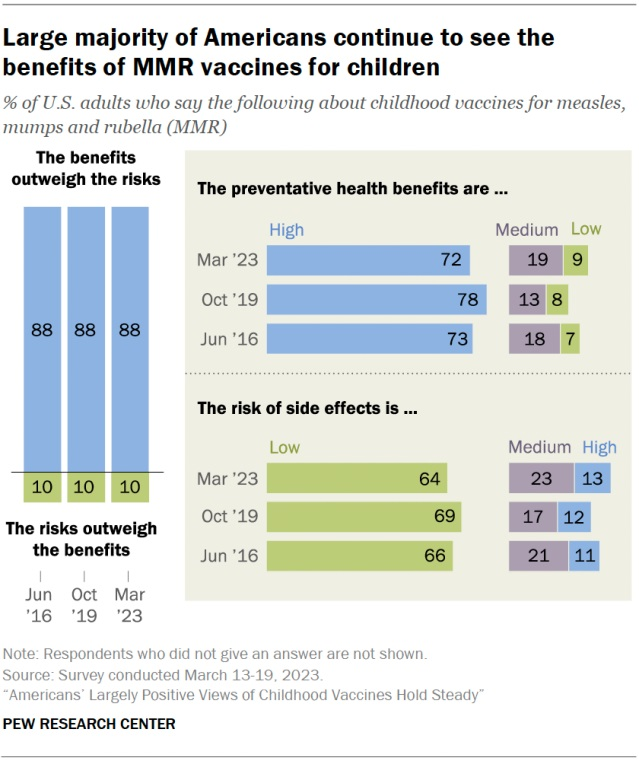
\includegraphics[width=400px]{../img/pew}

The Center survey finds 88\% of Americans say the benefits of childhood
vaccines for measles, mumps and rubella (MMR) outweigh the risks,
compared with just 10\% who say the risks outweigh the benefits.

The sample proportion of 0.88 is an estimate of the population
proportion. That is, the actual proportion of U.S. adults that believe
the benefits outweigh the risks.

Of course this is a single number estimate that would change if we
sampled again. We can report the standard deviation of this sample
proportion, called a standard error, to give us an idea of the
variability in the estimate.

Assuming independence between study participants, we can find an
estimated standard error for this sample proportion using techniques
learned earlier:

\[\widehat{SE(\hat{p})} = \sqrt{\frac{\hat{p}(1-\hat{p})}{n}} \approx \sqrt{\frac{0.88*0.12}{10701}} = 0.0031\]
Two big questions arise:

\begin{itemize}
\tightlist
\item
  First, can we provide a range of values we are `confident' the true
  proportion falls in?

  \begin{itemize}
  \tightlist
  \item
    We need to know about more than just the variability of the
    estimator
  \item
    We need to understand the \textbf{distribution} of the estimator!

    \begin{itemize}
    \tightlist
    \item
      Called the \textbf{sampling distribution}
    \item
      Describes the pattern in which we observe this \(\hat{p}\)
    \end{itemize}
  \item
    The sampling distribution can be difficult to derive in some cases!
  \end{itemize}
\item
  Second, does our estimator \(\hat{p}\) get closer to the true value
  \(p\) for larger sample sizes?

  \begin{itemize}
  \tightlist
  \item
    That is, does \(\hat{p}\) \emph{converge} to \(p\) as n grows?
  \item
    What does it even mean for a random quantity to converge?
  \end{itemize}
\end{itemize}

These two questions can often be answered by looking at the
\emph{limiting} behavior (here as the sample size grows) of the
estimator \(\hat{p}\).

\hypertarget{stackreldrightarrow-idea}{%
\subsection{\texorpdfstring{\(\stackrel{d}{\rightarrow}\)
Idea}{\textbackslash stackrel\{d\}\{\textbackslash rightarrow\} Idea}}\label{stackreldrightarrow-idea}}

To answer the first question: ``Can we provide a range of values for the
parameter?'', let's consider determining the \emph{sampling
distribution} through simulation. A distribution just describes the
pattern in which we observe our variable. If we can simulate observing
the variable, we can create many \emph{realizations} of \(\hat{p}\) to
understand the \emph{sampling distribution}.

To do this we need to make some assumptions. Namely:

\begin{itemize}
\tightlist
\item
  We have \(n\) \(iid\) (independent and identically distributed) trials
\item
  A value for the true \(p\)
\end{itemize}

Let's use the app below to consider the sampling distribution when \(p\)
is 0.9 and \(n\) is 10.

Instructions:

\begin{itemize}
\tightlist
\item
  ``n: sample size'' Slider: Move the slider to the right to increase
  the sample size
\item
  ``p: true value in population'' Slider: Move the slider to the right
  to increase the true proportion
\item
  ``Generate a sample proportion'': Click this button to add a single
  randomly generated sample proportion to the plot
\item
  ``Generate 100 sample proportions'': Click this button to add 100
  randomly generated sample proportions to the plot
\item
  ``Add +/- 2 Standard Error and Overlay Smoothed Density'' Check this
  bot to add bars corresponding to two standard errors and also add a
  smoothed density overlayed
\end{itemize}

Put your thoughts from using the app here!

As long as the distribution is roughly normal, we can see that 0.95 of
the distribution falls within two standard errors of \(p\). For 95\% of
the \(\hat{p}\) values we observe, adding and subtracting two standard
errors would capture the true \(p\). This means we could use something
like

\[\hat{p}\pm 2*\widehat{SE(\hat{p})}\]

as an interval to \emph{capture} the true \(p\). (Indeed this is the
usual basic interval for a proportion!)

\hypertarget{stackrelprightarrow-idea}{%
\subsection{\texorpdfstring{\(\stackrel{p}{\rightarrow}\)
Idea}{\textbackslash stackrel\{p\}\{\textbackslash rightarrow\} Idea}}\label{stackrelprightarrow-idea}}

To answer the second question: ``does our estimator \(\hat{p}\) get
closer to the true value \(p\) for larger sample sizes?'', we could
consider generating sample proportions for ever increasing values of the
sample size and seeing how they behave. Using the app below, we can
generate many sample proportions for varying \(n\), subtract off the
true value of \(p\), and see how that difference changes on the plot.

\begin{itemize}
\tightlist
\item
  Start with one sample proportion at each \(n\) and see the behavior of
  \(\hat{p}-p\).
\item
  Now increase the number of sample proportions generated for each
  \(n\). What aspect of this relationship does this help us understand?
\item
  Increase the sample size you are considering. What happens to the
  observed difference as \(n\) grows?
\end{itemize}

Instructions:

\begin{itemize}
\tightlist
\item
  ``Maximum Sample Size'': Enter a number to increase/decrease the
  largest sample size to consider
\item
  ``\# samples at each n'' Slider: Move the slider to select the number
  of sample proportions to generate at each given sample size
\item
  ``p: true value in population'': Move this slider to select the true
  proportion from the population
\item
  ``Create/Update graph'': Click this button to create the initial graph
  or update the graph based off of new selections of the above values
\end{itemize}

Put your thoughts from using the app here!

We can see that \(\hat{p}-p\) seems to get closer to 0. This indicates
that \(\hat{p}\) is in some sense \emph{converging} to the true value of
\(p\)!

Now that we some basic intuition, let's formalize what we are talking
about.

\hypertarget{definitions}{%
\subsection{Definitions}\label{definitions}}

By \emph{limit}, \emph{large-sample}, or \emph{asymptotic} theory we
mean we want to understand the behavior of some quantity, usually a
\emph{statistic}, as something changes, usually the sample size \(n\).
For instance, we will investigate the behavior of the sample mean,
\(\bar{Y}\), as the sample size grows. We'll look at questions like:

\begin{itemize}
\tightlist
\item
  When the distribution of a statistic (called a \textbf{sampling
  distribution}) is difficult to derive \emph{exactly}, is there a good
  \textbf{approximating} distribution that can be used to get
  \textbf{approximate} probability statements about \(\bar{Y}\)?
\item
  What value does \(\bar{Y}\) \emph{get close to} or \emph{converge to}
  as the sample size grows?
\end{itemize}

Answers to these questions will allows us to do inference (confidence
intervals and hypothesis tests) and understand the quality of our
estimator.

\hypertarget{common-assumptions-definitions}{%
\subsubsection{Common Assumptions \&
Definitions}\label{common-assumptions-definitions}}

We often make some assumptions about how we observe our random variables
in order to investigate these types of questions. For simplicity, we
often assume we have a \textbf{random sample}.

\begin{description}
\tightlist
\item[Random Sample]
\(Y_1,..., Y_n\) are a random sample (RS) of size \(n\) if the random
variables are independent and identically distributed (iid).
\end{description}

We'll often say `assume we have a random sample' from some distribution
or that `our random variables are iid' from some distribution. These are
equivalent ways of stating this assumption.

For the proportion example mentioned previously, we might formally state
our assumption as follows:

\begin{itemize}
\tightlist
\item
  Define
  \(X_i = \begin{cases} 1 & \mbox{if the }i^{th}\mbox{ individual says the benefits of childhood vaccines for MMR outweigh the risks}\\ 0 & \mbox{if not}\end{cases}\)
\item
  Then \(X_i\stackrel{iid}\sim Ber(p)\) where \(p\) represents the true
  proportion of people in the U.S. that believe the benefits outweight
  the risks
\item
  The random variable \(Y = \sum_{i=1}^{n}X_i \sim Bin(n,p)\)
\item
  We then often try to use \(Y\) or \(\hat{p}=Y/n\) to make inference on
  \(p\).
\item
  \(Y\) and \(\hat{p}\) are referred to as \textbf{statistics}. Note:
  \(\hat{p}\) is also \(\bar{X}\)!
\end{itemize}

\begin{description}
\tightlist
\item[Statistic]
A function of \(Y_1,Y_2,...,Y_n\) from a random sample that does not
involve any unknown parameters is called a statistic.
\end{description}

Commonly studied statistics:

\begin{itemize}
\tightlist
\item
  \(\bar{Y} = \frac{1}{n}\sum_{i=1}^n Y_i\)
\item
  \(S^2 = \frac{1}{n-1}\sum_{i=1}^{n}(Y_i-\bar{Y})^2\)
\item
  \(Y_{(n)} = \mbox{the maximum value from the sample}\)
\end{itemize}

Quantities that aren't statistics:

\begin{itemize}
\tightlist
\item
  \(\frac{\bar{Y}-\mu}{S/\sqrt{n}}\) (since \(\mu\) is unknown - if we
  assume \(\mu\) is known (like when we do in a hypothesis test) then
  this is a statistic)
\item
  \(\frac{(n-1)S^2}{\sigma^2}\) (since \(\sigma^2\) is unknown)
\end{itemize}

One type of convergence we'll look at is focused on the pattern in which
these statistics are observed, that is, the \textbf{sampling
distribution} of the statistics.

Recall that a distribution is just the pattern and frequency with which
we observe a random variable. With a statistic, we give this
distribution the special name of \textbf{sampling distribution}. This is
because we can think of how that distribution is formed by considering
repeated samples from the population, each sample producing the
statistic of interest.

\begin{description}
\tightlist
\item[Sampling Distribution]
The distribution of a statistic is called a sampling distribution.
\end{description}

We see that the sampling distribution of \(\hat{p}\) looks like a bell
curve for some combinations of \(n\) and \(p\). If we fix a \(p\) and
increase \(n\), we will start to see a bell shape for large enough
\(n\)! Later we'll see that a good \textbf{large-sample} distribution
for \(\hat{p}\) is the Normal distribution with mean \(p\) and variance
\(p(1-p)/n\).

We can see that there may be a distinction between the \emph{actual}
distribution, which is a discrete distribution for \(\hat{p}\), and an
approximating distribution, the Normal distribution for \(\hat{p}\). We
call these by different names.

\begin{description}
\tightlist
\item[Exact Distribution]
The (sampling) distribution of a quantity that is valid for any sample
size (or, occasionally, values of the parameters of the population
distribution).
\item[Large-Sample or Approximate Distribution]
A (sampling) distribution that is reasonable to use for a quantity for a
\emph{large} sample size (or occasionally other parameter values).
\end{description}

We use the notation \[Statistic \stackrel{\bullet}\sim f\] to denote a
large-sample approximating distribution.

In the sample proportion example, we would write

\[\hat{p}\stackrel{\bullet}\sim N(p, p(1-p)/n)\]

\hypertarget{convergence-in-distribution}{%
\subsection{Convergence in
Distribution}\label{convergence-in-distribution}}

While convergence in distribution can be visually inspected with a
histogram, to formally define \textbf{convergence in distribution} we
use the cumulative distribution function or CDF.

Recall the Cumulative Distribution Function (or CDF) of a random
variable \(Y\) is defined as

\[F_Y(y) = P(Y\leq y)\] For our binomial example, we can compare the CDF
of binomial random variables to Normal random variables to see that the
Binomial is `converging' to the normal distribution in a sense!

\includegraphics[width=400px]{ConvergenceConceptsNotesToPDF_files/figure-latex/unnamed-chunk-2-1}

\includegraphics[width=400px]{ConvergenceConceptsNotesToPDF_files/figure-latex/unnamed-chunk-3-1}

\begin{description}
\tightlist
\item[Convergence in Distribution]
Consider a sequence of random variables \(Y_1,...,Y_n,...\) with
corresponding CDFs \(F_{Y_1}(y), ..., F_{Y_n}(y),..\). Then \(Y_n\)
converges in distribution to the random variable \(Y\) (with CDF
\(F_Y(y)\)) if \[\lim_{n \rightarrow \infty} F_{Y_n}(y)=F_{Y}(y)\] or
equivalently \[\lim_{n \rightarrow \infty} |F_{Y_n}(y)-F_{Y}(y)|=0\] (at
all points \(y\) where \(F_Y(y)\) is continuous). We denote this as
\[Y_n\stackrel{d}\rightarrow Y\]
\end{description}

The subscript \(n\) notation here may be confusing. This is just to show
the RV on the left is dependent on the sample size in some way. For our
example with a Binomial/sample proportion, the distribution clearly
depends on \(n\). We could write the following to be explicit:

\[Y_n \sim Bin(n, p)\mbox{   and   } \hat{p}_n = Y_n/n\]

We'll prove (via the CLT) that the standardized version of these
statistics converge to a standard Normal distribution! For example,
\[Z_n = \frac{\hat{p}_n-p}{\sqrt{p(1-p)/n}} \stackrel{d}{\rightarrow}Z\sim N(0,1)\]

Alternatively, for practical purposes we'll equivalently talk about
`large-sample' distributions using the \(\stackrel{\bullet}{\sim}\)
notation:
\[\hat{p}_n\stackrel{\bullet}{\sim}N\left(p, \frac{p(1-p)}{n}\right)\]
It is sometimes easier to work with MGFs rather than CDFs. In that case,
we can use the following result:

\begin{description}
\tightlist
\item[Convergence of MGFs]
Consider a sequence of random variables \(Y_1,...,Y_n,...\) with
corresponding MGFs \(m_{Y_1}(t), ..., m_{Y_n}(t),..\). Then \(Y_n\)
converges in distribution to the random variable \(Y\) (with MGF
\(m_Y(t)\)) if \[\lim_{n \rightarrow \infty} m_{Y_n}(t) = m_Y(t)\]
\end{description}

\hypertarget{proving-stackreldrightarrow-using-cdfs}{%
\subsubsection{\texorpdfstring{Proving \(\stackrel{d}\rightarrow\) using
CDFs}{Proving \textbackslash stackrel\{d\}\textbackslash rightarrow using CDFs}}\label{proving-stackreldrightarrow-using-cdfs}}

\textbf{Example:} Suppose that \(Y_i\stackrel{iid}\sim U(0,1)\). That
is, \[f_Y(y) = \begin{cases}1 & 0<y<1\\0 & otherwise\end{cases}\] and
\[F_Y(y) = \begin{cases} 0 & y < 0\\ y & 0\leq y < 1 \\ 1 & y\geq 1\end{cases}\]
What does the maximum from the sample converge to in distribution as
\(n\) grows?

Let's generate many samples, find the maximum for each sample, and look
at the empirical distribution via a histogram and CDF.

\includegraphics{ConvergenceConceptsNotesToPDF_files/figure-latex/unnamed-chunk-4-1.pdf}
\includegraphics{ConvergenceConceptsNotesToPDF_files/figure-latex/unnamed-chunk-4-2.pdf}

It appears that the distribution converges to a random variable that
always takes on 1. We'd say there is a \textbf{point mass} at 1. If
\(W\) is a random variable that always takes on the constant \(c\) then
\[f_W(w) = \begin{cases} 1 & w = c\\ 0 & otherwise\end{cases}\]
\[F_W(w) = \begin{cases} 0 & w < c\\ 1 & w\geq c\end{cases}\]

We also said we could look at
\[\lim_{n \rightarrow \infty} |F_{Y_n}(y)-F_{Y}(y)|=0\] for convergence
in distribution. This difference in CDFs can be plotted in three
dimensions.

\includegraphics{ConvergenceConceptsNotesToPDF_files/figure-latex/unnamed-chunk-5-1.pdf}

Let's formally prove that the maximum of \(n\) iid \(U(0,1)\) RVs
converges to a RV with a point mass at 1.

\textbf{Example:} Consider again a random sample of \(U(0,1)\) RVs. What
does \(W = n(1-Y_{(n)})\) converge in distribution to as \(n\) grows?
Can we describe a rule of thumb for when the approximating distribution
is reasonable?

\includegraphics{ConvergenceConceptsNotesToPDF_files/figure-latex/unnamed-chunk-6-1.pdf}
\includegraphics{ConvergenceConceptsNotesToPDF_files/figure-latex/unnamed-chunk-6-2.pdf}

This one doesn't appear to be converging to a point mass. Let's use the
limit of the CDF to determine what this random variable converges to.

Let's compare the distribution of \(W = n(1-Y_{(n)})\) with
\(X \sim exp(1)\) via a plot of \[|F_{Y_n}(y)-F_{Y}(y)|\]

\includegraphics{ConvergenceConceptsNotesToPDF_files/figure-latex/unnamed-chunk-7-1.pdf}

\hypertarget{proving-stackreldrightarrow-using-mgfs}{%
\subsubsection{\texorpdfstring{Proving \(\stackrel{d}\rightarrow\) using
MGFs}{Proving \textbackslash stackrel\{d\}\textbackslash rightarrow using MGFs}}\label{proving-stackreldrightarrow-using-mgfs}}

\textbf{Example:} Suppose \(Y\sim Bin(n,p)\) where
\(np \rightarrow \lambda\) as \(n\) grows. Show
\(Y\stackrel{d}\rightarrow Poi(\lambda)\).

First, let's compare plots to see that the relationship seems to hold.
We'll create three different binomial and poisson plots with the same
ratio for \(n\) and \(p\).

Consider how well do the PMFs match up for the following situations:

\begin{itemize}
\tightlist
\item
  \(n = 10, p = 0.5 \rightarrow n*p = 5\)
\end{itemize}

\includegraphics{ConvergenceConceptsNotesToPDF_files/figure-latex/unnamed-chunk-9-1.pdf}

\begin{itemize}
\tightlist
\item
  \(n = 100, p = 0.05 \rightarrow n*p = 5\)
\end{itemize}

\includegraphics{ConvergenceConceptsNotesToPDF_files/figure-latex/unnamed-chunk-10-1.pdf}

\begin{itemize}
\tightlist
\item
  \(n = 1000, p = 0.005 \rightarrow n*p = 5\)
\end{itemize}

\includegraphics{ConvergenceConceptsNotesToPDF_files/figure-latex/unnamed-chunk-11-1.pdf}

\textbf{Example:} After we learn about the central limit theorem (CLT),
we'll see a (relatively) easy way to prove that a
\(Y\sim Gamma(n, \lambda)\), properly standardized, converges to a
standard normal distribution. That is,
\[W = \frac{Y-n/\lambda}{\sqrt{n}/\lambda}\stackrel{d}{\rightarrow} Z \sim N(0,1)\]
We can prove it using MGFs directly. Let's look through the proof below:

Goal: Start with the MGF of the standardized random variable and try to
show it converges to a standard normal MGF (\(e^{t^2/2}\)) as
\(n\rightarrow\infty\).

\begin{align*} 
m_Z(t) &= E\left(e^{t\left(\frac{Y-n/\lambda}{\sqrt{n}/\lambda}\right)}\right)\\
       &= E\left(e^{\frac{t\lambda}{\sqrt{n}}Y}\right)e^{-t\sqrt{n}}\\
       &= \left(\frac{1}{1-\frac{(\lambda t)/\sqrt{n}}{\lambda}}\right)^{n}e^{-t\sqrt{n}}\\
       &= \left(\frac{e^{-t/\sqrt{n}}}{1-t/\sqrt{n}}\right)^{n}\\
\end{align*}

As we want the limit of this quantity as \(n\) goes to infinity,
consider that this involves \(n\) in the term and is raised to the
\(n\). We saw the result:

\[\lim_{n\rightarrow\infty}(1+a_n/n)^n=e^a\] where
\(\lim_{n\rightarrow\infty}a_n=a\). A rewrite can allow us to use this!

\begin{align*}
      &= \left(1+\frac{n\left(\frac{e^{-t/\sqrt{n}}}{1-t/\sqrt{n}}-1\right)}{n}\right)^{n}\\
\end{align*}

Now we can just consider what happens to the numerator of the second
term as \(n\) grows. That is, we just need to consider
\[\lim_{n\rightarrow\infty}n\left(\frac{e^{-t/\sqrt{n}}}{1-t/\sqrt{n}}-1\right)\]
Using a common denominator and then applying a Taylor series expansion
of the \(e\) term about 0,
\[e^{-t/\sqrt{n}}=1-t/\sqrt{n}+t^2/(2n)-t^3/(3!n^{3/2})+...,\] we can
rewrite this as \begin{align*}
    &= \lim_{n\rightarrow\infty}n\left(\frac{t^2/(2n)-t^3/(3!n^{3/2})+...}{1-t/\sqrt{n}}\right)\\
    &= \lim_{n\rightarrow\infty}\left(\frac{t^2/2-t^3/(3!n^{1/2})+...}{1-t/\sqrt{n}}\right)\\
    &= t^2/2\\
\end{align*}

Thus, our MGF converges \(e^{t^2/2}\). This is the MGF of a standard
normal random variable! Therefore,

\[W = \frac{Y-n/\lambda}{\sqrt{n/\lambda^2}}\stackrel{d}{\rightarrow} Z \sim N(0,1)\]

\hypertarget{central-limit-theorem}{%
\subsubsection{Central Limit Theorem}\label{central-limit-theorem}}

One of the most important theorems in statistics is the Central Limit
Theorem (CLT). The CLT gives us a general result about the large-sample
behavior of a sample mean.

\begin{description}
\tightlist
\item[Central Limit Theorem (CLT)]
Suppose that \(Y_i\stackrel{iid}\sim f_Y\) where \(E(Y)=\mu\) and
\(Var(Y)=\sigma^2 < \infty\). Define
\(\bar{Y}=\frac{1}{n} \sum_{i=1}^{n} Y_i\) and \(Z \sim N(0, 1)\). Then
the standardized sample mean converges in distribution to a standard
normal random variable.
\[\frac{\bar{Y}-\mu}{\sigma/\sqrt{n}} \stackrel {d} {\rightarrow} Z\]
\end{description}

Practically, we can say that a good approximating distribution or
large-sample distribution for \(\bar{Y}\) is
\[\bar{Y}\stackrel{\bullet}\sim N(\mu, \sigma^2/n)\]

\hypertarget{clt-applied-to-a-sample-proportion}{%
\paragraph{CLT Applied to a Sample
Proportion}\label{clt-applied-to-a-sample-proportion}}

\textbf{Example:} A common application of the CLT is to the sample
proportion from a Binomial experiment.

For example, if \(X_i\stackrel{iid}\sim Bin(1, p)\) with mean
\(E(Y) = p\) and variance \(Var(Y) = p(1-p)\).

Define \(Y = \sum_{i=1}^n X_i\). We know \(Y\sim Bin(n, p)\). The sample
proportion is then \[\hat{p}=\frac{Y}{n} = \frac{\sum_{i=1}^n X_i}{n}\]
By the CLT, we can say that the sampling distribution of \(\hat{p}\) can
be well approximated by a Normal distribution with mean \(E(X_i) = p\)
and variance \(Var(X_i)/n = p(1-p)/n\).

We might state this as either

\[\frac{\hat{p}-p}{\sqrt{p(1-p)/n}} \stackrel{d}\rightarrow Z\sim N(0,1)\]
or

\[\hat{p}\stackrel{\bullet}\sim N(p, p(1-p)/n)\]

You've likely seen the Normal approximation to the Binomial before. You
may even know a rule of thumb for using it. The app below simulates
sample proportions from a given binomial distribution. Use the app below
to

\begin{itemize}
\tightlist
\item
  Explore the relationship between \(\hat{p}\) and the corresponding
  Normal distribution (the larger the \(M\) value the more precisely the
  graph mimics the exact distribution of \(\hat{p}\))
\item
  Either verify the rule of thumb you know or try and come up with a
  rule of thumb for when the approximation is reasonable
\end{itemize}

Put your thoughts from using the app here!

\hypertarget{clt-applied-to-a-sum}{%
\paragraph{CLT Applied to a Sum}\label{clt-applied-to-a-sum}}

Recall the result:

\begin{itemize}
\tightlist
\item
  If \(X\sim N(\mu, \sigma^2)\) then \(aX+b\sim N(a\mu+b,a^2\sigma^2)\)
\end{itemize}

That is, a Normal random variable multiplied by a constant is still
Normally distributed, just with a different mean and variance. - This
tells us that if the CLT is applicable to the sample average, then we
can also apply it to the corresponding summation as well!

Under the same assumptions as the CLT, since
\(n\bar{Y} = \sum_{i=1}^{n}Y_i\) we have the following result:
\[\frac{\sum_{i=1}^{n} Y_i -n\mu}{\sqrt{n}\sigma}\stackrel{\bullet}{\sim}N(0, 1)\]
or

\[\sum_{i=1}^{n} Y_i \stackrel{\bullet}{\sim}N(n\mu, n\sigma^2)\]

\textbf{Example:} Based on this result, what is a good large-sample
distribution for \(Y\sim Bin(n, p)\)?

\hypertarget{clt-applied-to-a-gamma}{%
\paragraph{CLT Applied to a Gamma}\label{clt-applied-to-a-gamma}}

\textbf{Example:} Earlier we proved that \(Y\sim Gamma(n, \lambda)\),
properly standardized, converges to a standard normal distribution. That
is,
\[W = \frac{Y-n/\lambda}{\sqrt{n}/\lambda}\stackrel{d}{\rightarrow} Z \sim N(0,1)\]

Rather than use MGFs, we can apply the CLT in a clever way!

First, note that for \(Y\sim gamma(n,\lambda)\) we can think of \(Y\) as
\(Y=X_1+X_2+...+X_{n}\), where
\(X_i\stackrel{iid}\sim gamma(1,\lambda)\). Here we know that
\(E(X_i) = 1/\lambda\) and \(Var(X_i) = 1/\lambda^2\). By the CLT
applied to a sum we know

\[\frac{\sum_{i=1}^{n} X_i -n(1/\lambda)}{\sqrt{n}(1/\lambda)} = \frac{Y-n/\lambda}{\sqrt{n/\lambda^2}}\stackrel{\bullet}{\sim}Z\]

where \(Z\sim N(0,1)\). That means we can approximate a gamma random
variable by \[Y \stackrel{\bullet}{\sim} N(n/\lambda, n/\lambda^2)\]

Alternatively, we could apply the CLT to an average instead of a sum.
Instead use \(X_i\stackrel{iid}{\sim}gamma(1,\lambda/n)\) then \(Y\) can
be thought of as an average of these \(X\)'s
\[Y=\frac{1}{n}\sum_{i=1}^{n}X_i=\bar{X}\sim gamma(n,\lambda)\] We know
that \(E(X_i) = n/\lambda\) and \(Var(X_i) = n^2/lambda^2\). Since we
are now viewing this as an average of iid random variables we can apply
the CLT.\\
\[\frac{\bar{X}-n\lambda}{\sqrt{(n^2/\lambda^2)/n}}=\frac{\bar{X}-n\lambda}{\sqrt{n/\lambda^2}}\stackrel{d}\rightarrow Z\]
where \(Z\sim N(0,1)\).

\hypertarget{convergence-exploration}{%
\subparagraph{Convergence Exploration}\label{convergence-exploration}}

\begin{itemize}
\tightlist
\item
  Suppose that \(Y \sim Gamma(n, \lambda)\). Or, assume that
  \(Y = \sum_{i=1}^{n} X_i\) where
  \(X_i\stackrel{iid}\sim Gamma(1, \lambda)\).
  \[f_Y(y) = \frac{\lambda^\alpha}{\Gamma(\alpha)}y^{\alpha -1}e^{-\lambda y}\]
  with mean \(E(Y) = \alpha/\lambda\) and variance
  \(Var(Y) = \alpha/\lambda^2\).
\item
  We again showed we can approximate a gamma by a Normal distribution.\\
\item
  Can you develop a rule of thumb around \(\alpha\) (\(n\) here) and
  \(\lambda\) for when a Normal distribution may be a reasonable
  approximation? Remember we look for the following in each graph:

  \begin{itemize}
  \tightlist
  \item
    Histogram: when does it become a symmetric bell-shape?
  \item
    CDF comparison: When do the CDFs essentially overlap?
  \end{itemize}
\end{itemize}

Put your thoughts from using the app here!

\hypertarget{clt-importance}{%
\subsubsection{CLT Importance}\label{clt-importance}}

Practically, why is the CLT so important?

\begin{itemize}
\tightlist
\item
  The CLT gives us a distribution we can use to find probabilities when
  we deal with most sample sums and sample means.
\item
  Knowing a large-sample distribution allows us to find (approximate)
  probabilities when exact probabilities may be too difficult to find.
\item
  This means we can do approximate inference in many cases!
\end{itemize}

\textbf{Example:}

\begin{itemize}
\tightlist
\item
  Suppose we know \(\sigma\) and we want inference for \(\mu\).
\item
  If we have a random sample \(Y_1,...,Y_n\), we know
  \(\bar{Y}\stackrel{\bullet}{\sim}N(\mu,\sigma^2/n)\) (\(\mu\) only
  unknown)
\item
  We can make an approximate claim about \(\mu\) via a confidence
  interval derived from an argument similar to that below:
\end{itemize}

\begin{align*}
P(-1.96<Z<1.96) &= 0.95\\
\Leftrightarrow P\left(-1.96<\frac{\bar{Y}-\mu}{\sigma/\sqrt{n}}<1.96\right) &= 0.95\\
\Leftrightarrow P\left(\bar{Y}-1.96\sigma/\sqrt{n}<\mu<\bar{Y}+1.96\sigma/\sqrt{n}\right) &= 0.95\\
\end{align*}

\begin{itemize}
\tightlist
\item
  That is, there is a 95\% probability the RVs
  \(\bar{Y}-1.96\sigma/\sqrt{n}\) and \(\bar{Y}+1.96\sigma/\sqrt{n}\)
  capture \(\mu\)!
\item
  In practice we observe a value for \(\bar{Y}\) as \(\bar{y}\). We then
  lose the ability to talk about probability but instead asy we are 95\%
  confident the observed interval contains \(\mu\).
\item
  Note: No assumption about \(Y\)'s distribution made other than finite
  variance!
\end{itemize}

\hypertarget{convergence-in-probability-in-progress}{%
\subsection{Convergence in Probability
(in-progress)}\label{convergence-in-probability-in-progress}}

\end{document}
